\documentclass[a4paper,12pt,titlepage,twocolumn]{article}
\title{Phiếu ôn tập Lý phần LTAS \& VLHN viết bằng \textbf{\LaTeXe}}
\date{\today}
\author{Tạ Chí Thành Danh}
\usepackage[utf8]{vietnam} % Unicode tiếng Việt
\usepackage{amsmath}
\usepackage{amsfonts}
\usepackage{amssymb}
\usepackage{graphicx} % Dùng để chèn hình
\usepackage{textcomp}
\usepackage{hyperref}
\usepackage{enumitem} % Dùng để ghi hoa item của enumerate và chỉnh khoảng cách dòng item (setlist các thứ)
\usepackage{tipa} % Ngựa ngựa viết epsilon phiên bản Word =))) 
\usepackage{siunitx} % for SI Units
\usepackage[left=1cm,right=1cm,top=1.6cm,bottom=1cm]{geometry} % Định dạng khoảng cách lề giấy
\usepackage[fontsize=13pt]{scrextend} % Chỉnh cỡ chữ thành 13 như mặc định bên Word
\usepackage{tabularx} % Thư viện cho phép chèn itemize trong table
\usepackage{changepage} % for adjustwidth
\usepackage{setspace} % Linespacing
\usepackage{array} % for using {m|1cm|}
\usepackage{upgreek} % \uplambda
\usepackage{mathtools} % for prescript: https://www.overleaf.com/learn/latex/Articles/Mathtools_-_for_beautiful_math
%\usepackage{newtxtext,newtxmath} % Muốn dùng Times New Roman thì nhét cái này
\usepackage{fancyhdr} % dùng để tùy biến header theo ý mình
% Reference: https://www.overleaf.com/learn/latex/Headers_and_footers#Style_customization_in_single-sided_documents
\pagestyle{fancy}
\fancyhf{}
\lhead{Vật lý 12}
\chead{Biên soạn bằng \LaTeXe}
\rhead{\thepage}
\setlength{\columnseprule}{0.4pt} % Tạo một đường thẳng đứng ở giữa các cột
\newenvironment{myitemize} 
{ \begin{itemize}[leftmargin=*,label=-]  % https://www.overleaf.com/learn/latex/Environments
		% https://tex.stackexchange.com/questions/13463/specifying-bullet-type-when-using-itemize
		% Set new environment for itemize, source here: https://tex.stackexchange.com/questions/10684/vertical-space-in-lists
		\setlength{\itemsep}{0pt}
		\setlength{\parskip}{0pt}
		\setlength{\parsep}{0pt}     }
{ \end{itemize}                  } 
\newenvironment{myenumerate}
{ \begin{enumerate}[label=\textbf{\arabic*}.]
\setlist{nolistsep} % Xóa khoảng cách giữa enumerate và itemize
\setlength{\itemsep}{0pt}
\setlength{\parskip}{0pt}
\setlength{\parsep}{0pt}	}
{ \end{enumerate}}
% Muốn chỉnh lại kí hiệu lambda thì dùng 2 dòng này
%\DeclareSymbolFont{myletters}{OML}{ztmcm}{m}{it}
%\DeclareMathSymbol{\uplambda}{\mathord}{myletters}{"15}

% Render MeV/c^2: https://tex.stackexchange.com/questions/356334/rendering-mev-c%C2%B2-with-siunitx
\DeclareSIUnit\eVperc{\eV\per\clight}
\DeclareSIUnit\clight{\text{\ensuremath{c}}}

% https://tex.stackexchange.com/questions/350453/z-with-a-stroke-through-it
%\newcommand{\zbar}{%
%	\text{\ooalign{\hidewidth\raisebox{0.2ex}{--}\hidewidth\cr$Z$\cr}}%
%}

\begin{document}
	%\maketitle
Lớp: 12A7 \quad Họ tên: Tạ Chí Thành Danh \\
\begin{adjustwidth}{-0.2cm}{}
	\begin{center}
		\small\textbf{ÔN TẬP CHƯƠNG LƯỢNG TỬ ÁNH SÁNG}
	\end{center}
\end{adjustwidth}
\begin{myenumerate}
	\item \textbf{Lượng tử năng lượng là} lượng năng lượng mỗi lần nguyên tử \textbf{hấp thụ} hay \textbf{phát xạ} \\
		\textepsilon{} $=hf=\dfrac{hc}{\lambda}$ với $h=6,625 \cdot 10^{-34}$ \si{\joule\second}
	\item \textbf{Điều kiện có hiện tượng quang điện:} \\
	$\lambda \leqslant\ \lambda_0$; \textepsilon{} $\geqslant A$; $f \geqslant f_0$ \\
	Trong đó $A$ là \textbf{công thoát}, $\lambda_0$ là \textbf{giới hạn quang điện} với $\lambda_0 = \dfrac{hc}{A}$ \\
	Các công thức quang điện: 
	\begin{myitemize}
	\item[$\boldsymbol{\cdot}$ ]Cường độ dòng quang điện $I = n_e \cdot e$ \\ ($n_e$: $\mathrm{electrons}/s$)
	\item[$\boldsymbol{\cdot}$ ] Công suất chiếu sáng $P=n_p.$\textepsilon{} $=n_p.hf = n_p \cdot \dfrac{hc}{\lambda}$ ( $n_e$: $\mathrm{photons}/s$)
	\item[$\boldsymbol{\cdot}$ ] Hiệu suất quang điện $H = \dfrac{n_e}{n_p}$
	\end{myitemize}
	\item \textbf{So sánh hiện tượng quang điện trong và ngoài}
	\begin{myitemize}
		\item Giống nhau: muốn xảy ra thì $\lambda \leqslant\ \lambda_0$
		\item Khác nhau:
	\end{myitemize}
	\begin{adjustwidth}{-1cm}{}
	\renewcommand{\arraystretch}{0} 
	% Default value: 1, chỉnh xuống 0 để khoảng cách giữa các đường ngang với các dòng văn bản ngắn hơn
	\begin{tabular}{|p{4.3cm}|p{4.3cm}|}
		\hline
		Quang điện ngoài & Quang điện trong \\
		\hline
		\begin{myitemize}
			\item Xảy ra với \textbf{kim loại}
			\item ánh sáng thích hợp làm bật $e$ ra khỏi tấm \textbf{kim loại} 
			\item $\lambda_0$ nằm trong vùng \textbf{tử ngoại} 
			(riêng kim loại kiềm thì nằm vùng ánh sáng \textbf{nhìn thấy})
			\end{myitemize}
			&
			\begin{myitemize}
				\item Xảy ra với \textbf{chất bán dẫn}
				\item ánh sáng thích hợp giải phóng $e$ khỏi liên kết cộng hóa trị nhưng 
				$e$ vẫn nằm trong khối \textbf{chất bán dẫn}
				\item $\lambda_0$ nằm trong vùng \textbf{hồng ngoại}
			\end{myitemize}
		\\
		\hline
	\end{tabular}
	\end{adjustwidth}
	\item \textbf{Hiện tượng quang dẫn:} giảm \textbf{điện trở} của bán dẫn khi chiếu \textbf{ánh sáng} thích hợp
	\item \textbf{Quang điện trở và pin quang điện} hoạt động dựa trên hiện tượng \textbf{quang điện trong}
	\item \textbf{Thuyết lượng tử ánh sáng (thuyết photon):}
	\begin{myitemize}
		\item Ánh sáng là tạo bởi các hạt \textbf{photon} (lượng tử ánh sáng)
		\item Với mỗi as đơn sắc , các photon đều \textbf{mang năng lượng}, 
		mỗi photon mang năng lượng \textepsilon{} $=hf$
		\item Mỗi lần phân tử, nguyên tử phát xạ hay hấp thụ ánh sáng là phát xạ hay hấp thụ \textbf{photon}
		\item Các photon bay dọc theo tia sáng với \textbf{tốc độ ánh sáng}. \\
		\textit{Lưu ý: Photon chỉ tồn tại trong trạng thái \textbf{chuyển động}, không có photon đứng yên}
	\end{myitemize}
	\item \textbf{Tính chất của sóng ánh sáng:} lưỡng tính \textbf{sóng--hạt} \\
	Bước sóng càng dài, tính chất \textbf{sóng} thể hiện càng rõ: \textbf{giao thoa, nhiễu xạ, khúc xạ, tán sắc} \\
	Bước sóng càng ngắn, tính chất \textbf{hạt} thể hiện càng rõ: \textbf{quang điện, phát quang, ion hóa, khả năng đâm xuyên}
	\item \textbf{Mẫu nguyên tử Bo} 
	\begin{myitemize}
		\item Tiên đề về các trạng thái dừng: Nguyên tử chỉ tồn tại ở một số trạng thái có \textbf{năng lượng xác định}
		$E_m$, gọi là trạng thái dừng. Khi ở trạng thái dừng, nguyên tử \textbf{không bức xạ}.
	\end{myitemize}
	\begin{adjustwidth}{-0.9cm}{}
	%\renewcommand{\arraystretch}{0}
	\begin{tabular}{|m{2.4cm}|m{0.75cm}|m{0.75cm}|m{0.75cm}|m{0.75cm}|m{0.75cm}|m{1cm}|}
		\hline
		n & 1 & 2 & 3 & 4 & 5 & 6 \ldots \\ \hline
		Tên quỹ đạo & K & L & M & N & O & P \\ \hline
		Trạng thái & Cơ bản & KT1 & KT2 & KT3 & KT4 & KT5 \\ \hline	
	\end{tabular}
	\end{adjustwidth}
	Với Hidro, bán kính quỹ đạo dừng $r_n = n^2 \cdot r_0$ với $r_0 = 5,3 \cdot 10^{-11}$ \si{\meter}
	\begin{myitemize}
		\item Tiên đề về bức xạ và hấp thụ năng lượng:
		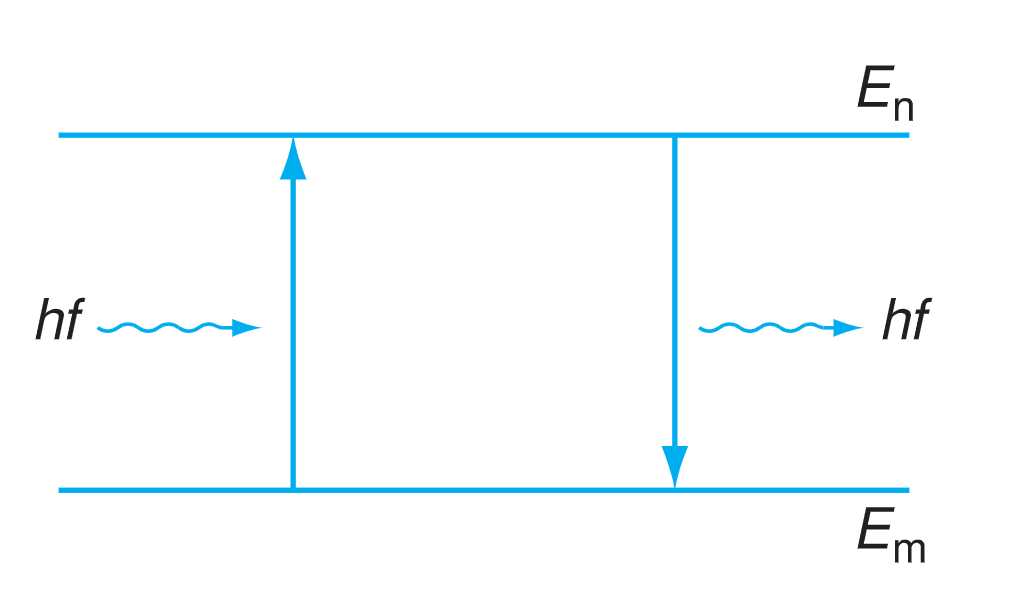
\includegraphics[scale=0.2]{image.png}
	\end{myitemize}
	\textepsilon{} $=hf=\dfrac{hc}{\lambda}=E_{n cao} - E_{m thấp}$ \\
	số vạch max $=\dfrac{n(n-1)}{2}$ \\
	$F = \dfrac{ke^2}{r^2} = ma_{ht} = \dfrac{mv^2}{r}$ \\
	Tia X: $\dfrac{hc}{\lambda_{min}} = hf_{max} = eU_{AK} = W_{\textit{đ}A}$
	\item \textbf{Quang phát quang}
	\begin{myitemize}
		\item Hấp thụ ánh sáng $\lambda$, phát ra ánh sáng $\lambda^\prime > \lambda$
		\item Huỳnh quang: ánh sáng phát quang \textbf{tắt ngay} sau khi tắt ánh sáng kích thích, thường xảy ra với \textbf{chất lỏng, khí}
		\item Lân quang: ánh sáng phát quang còn \textbf{kéo dài} sau khi tắt ánh sáng kích thích, thường xảy ra với \textbf{chất rắn} \\
	\end{myitemize} 
	\item \textbf{Laser}
	\begin{myitemize}
		\item Khuếch đại ánh sáng bằng \textbf{phát xạ cảm ứng}
		\item Đặc điểm của Laser:
		\setlength{\itemindent}{0.5cm} % Thụt cả câu vô 0.5cm
		\item[+] Tính \textbf{đơn sắc} rất cao: các photon có cùng $f$
		\item[+] Tính \textbf{kết hợp} cao: các photon cùng tần số, cùng pha.
		\item[+] Tính \textbf{định hướng} cao (là các chùm sáng song song): các photon bay theo cùng một phương.
		\item[+] Có \textbf{cường độ} lớn.
	\end{myitemize}
\end{myenumerate}	
\begin{adjustwidth}{-0.2cm}{}
	\begin{center}
		\small\textbf{ÔN TẬP CHƯƠNG VẬT LÝ HẠT NHÂN}
	\end{center}
\end{adjustwidth}
\begin{myenumerate}
	\item \textbf{Lực hạt nhân:} là \textbf{lực tương tác mạnh}, liên kết các nucleon trong hạt nhân,
	 bán kính tác dụng cỡ \textbf{kích thước hạt nhân} (khoảng $10^{-15}$ \si{\meter})
	\item \textbf{Hệ thức Einstein, độ hụt khối, năng lượng liên kết}
	\begin{myitemize}
		\item Hệ thức Einstein giữa khối lượng và năng lượng: $E=mc^2$ 
		\item Năng lượng toàn phần $=E_{\textit{nghỉ}} + W_{\textit{đ}}$ 
		\item Khối lượng động $m=\dfrac{m_0}{\sqrt{1-\dfrac{v^2}{c^2}}}$ 
		\item Đơn vị khối lượng của nguyên tử \\
		 $1u=\dfrac{1}{12} m$ nguyên tử $^{12}_6C=931,5$ \si[per-mode=symbol]{\mega\eVperc\squared} 
		 % per-mode=symbol để in ra dấu /
		 \item Độ hụt khối của hạt nhân $^A_ZX$: \\ $\Delta m = Z.m_p + (A-Z).m_n-m_X$
		 \item Năng lượng liên kết $W_{lk} = \Delta m.c^2$
		 \item Năng lượng liên kết riêng $W_{lkR} = \dfrac{\Delta mc^2}{A}$
	\end{myitemize}
	\textbf{Năng lượng liên kết riêng} càng \textbf{lớn} thì hạt nhân càng \textbf{bền}.
	Hạt nhân bền nhất có $50<A<80$
	\item \textbf{Phóng xạ}
	\begin{myitemize}
		\item Quá trình phóng xạ: tự phát, ngẫu nhiên, không điều khiển được, không phụ thuộc yếu tố bên ngoài.
		\item Là phản ứng \textbf{tỏa năng lượng}.
	\end{myitemize}
	\item \textbf{Các tia phóng xạ}
	\begin{myitemize}
		\item Tia $\upalpha$: bản chất là hạt nhân $^4_2He$
		\item Tia $\upbeta$: $\upbeta^{+}$ là \textit{positron} $\prescript{0}{+1}{e}$, $\upbeta^{-}$ là \\ \textit{electron} $\prescript{0}{-1}{e}$
		\item Tia $\upgamma$: bản chất là \textbf{sóng điện từ} với bước sóng rất ngắn, khả năng đâm \textbf{rất lớn} so với $\upalpha$, $\upbeta$. (Tia $\upgamma$ \textbf{đi kèm} với phát xạ $\upalpha$, $\upbeta$)
	\end{myitemize}
	\textit{Lưu ý: Tia $\mathit{\alpha,\beta}$ \textbf{lệch} trong điện trường và từ trường, còn tia $\mathit{\gamma}$ thì \textbf{không lệch}}
	\item \textbf{Định luật phóng xạ}
	\begin{adjustwidth}{-0.5cm}{}
		% https://tex.stackexchange.com/questions/588/how-can-i-change-the-margins-for-only-part-of-the-text
		\begin{myitemize}
			\item Số hạt phóng xạ (còn lại) ở thời điểm $t$: \\ 
			$N = N_0 \cdot 2^{\tfrac{-t}{T}}_{\phantom{i}} = N_0 \cdot e^{-\lambda t}$ %\phantom{i} tạo kí tự vô hình
			% https://www.tutorialspoint.com/tex_commands/phantom.htm
			\item Số hạt bị phân rã sau $t$: $\Delta N = N_0 \cdot (1-2^{\tfrac{-t}{T}}_{\phantom{i}})$
			\item Khối lượng chất phóng xạ (còn lại) ở thời điểm $t$: $m = m_0 \cdot 2^{\tfrac{-t}{T}}_{\phantom{i}}$
			% Further reading: 
			% https://tex.stackexchange.com/questions/4519/how-do-i-create-an-invisible-character
			\item Khối lượng chất phóng xạ bị phân rã sau thời gian $t$: $\Delta m = m_0 \cdot (1-2^{\tfrac{-t}{T}}_{\phantom{i}})$
			\item Liên hệ khối lượng $m$ và số hạt $N$: $m = \dfrac{N}{N_A} \cdot A$
		\end{myitemize}
	\end{adjustwidth}
	$X \rightarrow Y +$ \textit{tia phóng xạ} thì \\
	$\dfrac{N_Y}{N_X} = \dfrac{\Delta N}{N} = \dfrac{1-2^{\tfrac{-t}{T}}_{\phantom{i}}}{2^{\tfrac{-t}{T}}_{\phantom{i}}}$ \\
	$\dfrac{m_Y}{m_X} = \dfrac{N_Y}{N_X} \cdot \dfrac{A_Y}{A_X} = \dfrac{\Delta N}{N} \cdot \dfrac{A_Y}{A_X}$ \\
	$T$: chu kỳ bán rã \\
	Hằng số phóng xạ $\lambda = \dfrac{\ln 2}{T}$, $\lambda$ càng \textbf{lớn} thì phân rã càng \textbf{nhanh}. \\
	% Natural logarithm symbol: https://www.tutorialspoint.com/tex_commands/ln.htm
	$T$ và $\lambda$ \textbf{không phụ thuộc} yếu tố bên ngoài, chỉ phụ thuộc \textbf{bản chất} của chất phóng xạ
	\item \textbf{Bốn định luật bảo toàn trong phản ứng hạt nhân}
	\begin{myitemize}
		\item Bảo toàn \textbf{số nucleon A}
		\item Bảo toàn \textbf{điện tích Z}
		\item Bảo toàn \textbf{động lượng}
		\item Bảo toàn \textbf{năng lượng toàn phần}
	\end{myitemize}
	Năng lượng phản ứng: \\
	$\Delta E = (m_0-m) \cdot c^2 = W^{\prime}_{\textit{đ}} -  W_{\textit{đ}}$ \\ 
	$\text{\quad \phantom{a}} =(\Delta m_0- \Delta m) \cdot c^2$ \\
	$\Delta E>0$: Phản ứng \textbf{tỏa} năng lượng \\
	$\Delta E<0$: Phản ứng \textbf{thu} năng lượng \\
	Liên hệ động năng và động lượng: \\ 
	$W_{\textit{đ}} = \dfrac{mv^2}{2} = \dfrac{p^2}{2m}$
	\item \textbf{Phản ứng phân hạch:} Hạt nhân \textbf{nặng} vỡ thành {hai mảnh nhẹ hơn}. 
	Ví dụ: $\prescript{235}{92}{\text{U}}, \prescript{239}{94}{\text{Pu}}$
	\item \textbf{Phản ứng phân hạch dây chuyền} \\
	Gọi $k$ là hệ số nhân neutron
	\begin{myitemize}
		\item[$\ast$] \textit{Điều kiện có phản ứng dây chuyền:} \\
		$k \geqslant 1 \textit{ và } m \geqslant m_{\textit{tới hạn}}$
	\end{myitemize}
	\item \textbf{Phản ứng nhiệt hạch:} tổng hợp \textbf{hai hạt nhân nhẹ} thành \textbf{hạt nhân nặng hơn}. \\
	$\Rightarrow$ Đây là nguồn gốc năng lượng của mặt trời và các sao. Ví dụ: $\prescript{1}{1}{\text{H}}, \prescript{2}{1}{\text{D}},\prescript{3}{1}{\text{T}}$
\end{myenumerate}
\end{document}